%%% Local Variables:
%%% mode: latex
%%% TeX-master: t
%%% End:

\documentclass{beamer}
\usepackage[utf8]{inputenc}
\usepackage{xcolor}
\usepackage{tcolorbox}
\usepackage{hyperref}
\usepackage{esint}
\usepackage{soul}
\usepackage[alf]{abntex2cite}
\usepackage{lipsum}
\usepackage[brazilian,hyperpageref]{backref}
\usepackage{graphicx}
\usepackage{microtype}


\usebackgroundtemplate{

\includegraphics[width=\paperwidth,
height=\paperheight]{../Imagens/3.jpeg}}
\usecolortheme{beaver}
\usefonttheme{serif}
\usetheme{AnnArbor}



\mode<presentation>


  \title[Grupo 4]{\Huge{Apresentação grupo 4}}

  \author[Autores]{Andréia Mota \\
    \text{\scriptsize{amota@usp.br}}}

  \date[Data]{\scriptsize{Revestimentos anticorrosivos} \\ Escola de Engenharia de Lorena - USP}

 \begin{document}

\begin{frame}
  \titlepage
\end{frame}

{\usebackgroundtemplate{
\includegraphics[height=\paperheight]{../Imagens/Fundo2.jpg}}
\begin{frame}
\begin{tcolorbox}[colback=blue!5!white,colframe=blue!70!white,title=Introdução]
\begin{itemize}

  	  \item{Ambientes que necessitam de revestimentos anticorrosivos}
 	   \item{Elementos adicionados a revestimentos anticorrosivos}

            \begin{figure}[!htb]
              \begin{center}

                \caption{Exemplo peça oxidada}
                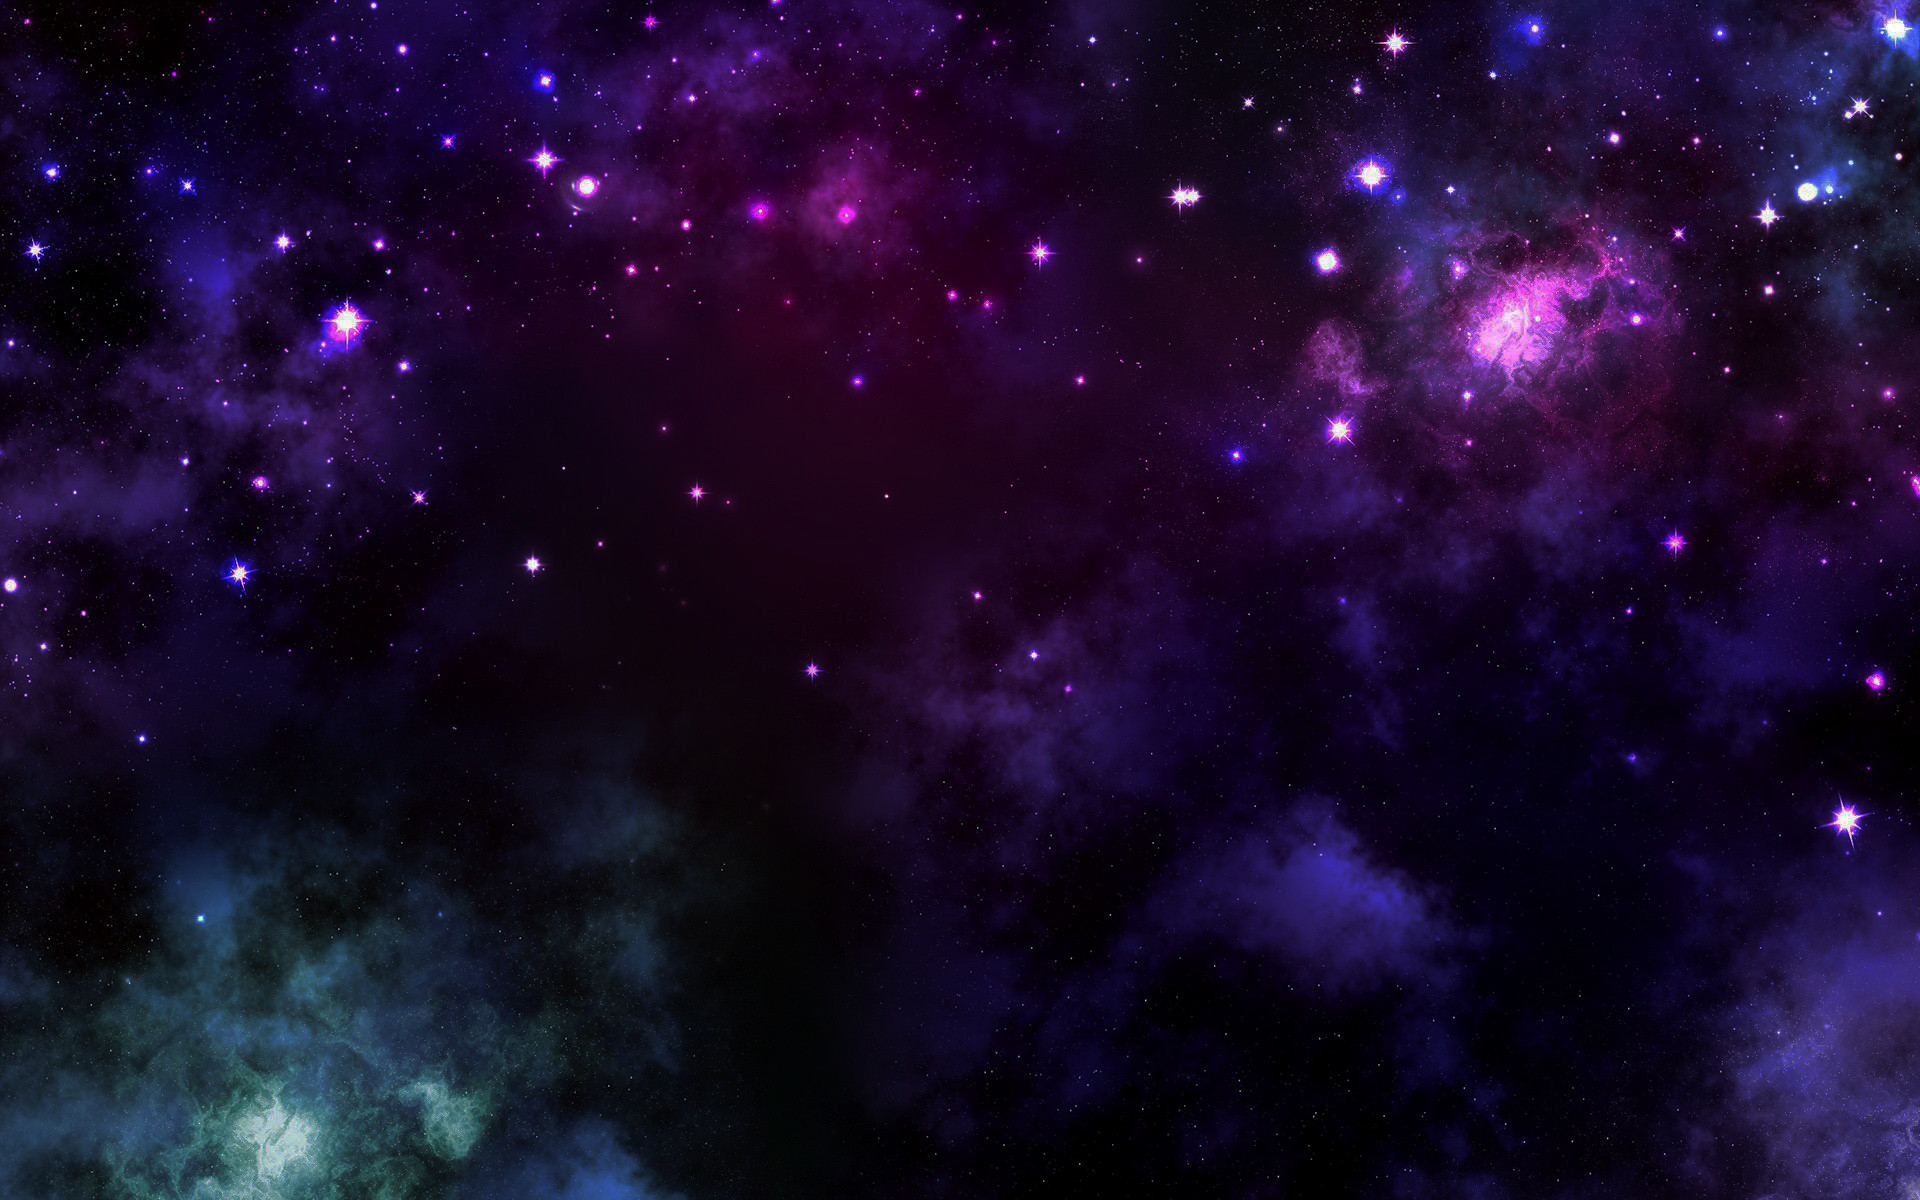
\includegraphics[width=0.7\linewidth]{../Imagens/Fundo1.jpg}
              \end{center}
              \legend{\cite{lidsky2009anonymity}}
            \end{figure}



\end{itemize}
\end{tcolorbox}
\end{frame}

\begin{frame}
  \frametitle{Referências}

  \bibliography{bib}

  \end{frame}
}
\end{document}
